\documentclass{article}

\renewcommand{\thesection}{}
\renewcommand{\thesubsection}{\arabic{section}.\arabic{subsection}}
\makeatletter
\def\@seccntformat#1{\csname #1ignore\expandafter\endcsname\csname the#1\endcsname\quad}
\let\sectionignore\@gobbletwo
\let\latex@numberline\numberline
\def\numberline#1{\if\relax#1\relax\else\latex@numberline{#1}\fi}
\makeatother

\newcommand{\senoide}{\mbox{$y = A\sin{(\omega x + \varphi)}$}}

\usepackage[utf8]{inputenc}

\title{Série de Fourier}
\author{Gustavo Higuchi}
\date{\today}

\usepackage{natbib}
\usepackage{graphicx}
\usepackage{amssymb}
\usepackage{amsthm}
\usepackage{amsmath}
\usepackage{color}   %May be necessary if you want to color links
\usepackage[portuguese, ruled, linesnumbered]{algorithm2e}
\usepackage{float}
\usepackage{pgfplots}
\usepgfplotslibrary{fillbetween}
\pgfkeys{/pgfplots/Axis Style/.style={
    width=13.5cm, height=5cm,
    axis x line=center, 
    axis y line=middle, 
    samples=200,
    ymin=-1.5, ymax=1.5,
    xmin=0, xmax=13.0,
    domain=0:4*pi
}}

\newtheorem{definicao}{Definição}
\newtheorem{teorema}{Teorema}

\theoremstyle{definition} 

\newtheorem*{exemplo}{Exemplo}


\usepackage{mathtools}
\DeclarePairedDelimiter\ceil{\lceil}{\rceil}
\DeclarePairedDelimiter\floor{\lfloor}{\rfloor}

% usado para linkar cada section na tabela de conteúdo com a respectiva
% página no documento
\usepackage{hyperref}
\hypersetup{
    colorlinks,
    citecolor=black,
    filecolor=black,
    linkcolor=black,
    urlcolor=black,
    linktoc=all
}

%o começo do documento
\begin{document}

% compila o título
\maketitle

% compila a tabela de conteúdos
\tableofcontents
\newpage

%
\chapter{Funções periódicas}

\begin{definicao}
\label{def1}
    
Uma função $f(x)$ é dita periódica se existe uma constante $T > 0$, tal que 
\begin{equation}
    f(x + T) = f(x)
\end{equation}
para qualquer $T \in \mathbb{R}$. 
\end{definicao}
Essa constante T é chamada de período da função $f(x)$. As funções periódicas 
mais comuns são $\sin{x}$, $\cos{x}$, $\tan{x}$, etc. Funções periódicas surgem
em muitas aplicações matemáticas e em problemas de física e engenharia. 
\\
Se plotarmos o gráfico da função $y=f(x)$ em qualquer intervalo fechado 
\mbox{$a \leq x \leq a + T$}, é possível obter o gráfico de $f(x)$ através da 
repitição periódica da porção do gráfico correspondente a \mbox{$a \leq x \leq a + T$}.
Na figura ~\ref{fig:periodExp}, temos uma função periódica de período $T=2\pi$.
\\
\begin{figure}[H]
    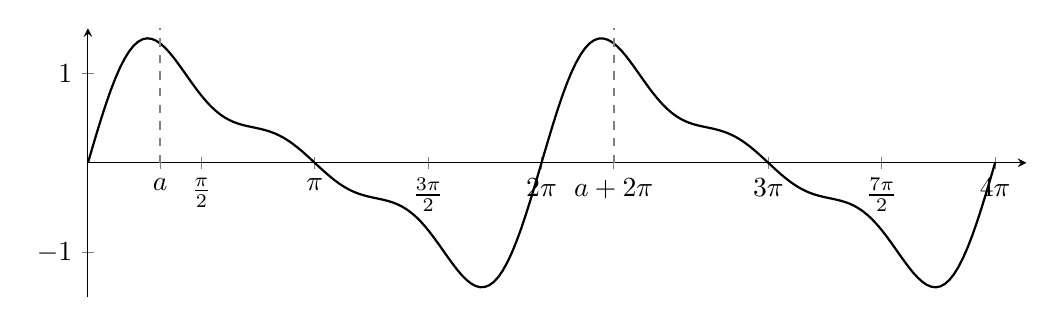
\begin{tikzpicture}
    \begin{axis}[
        Axis Style,
        xtick={
            -6.28318, -4.7123889, -3.14159, -1.5708, 1,
            1.5708, 3.14159, 4.7123889, 6.28318, 7.28318, 
            9.42478, 10.99558, 12.56638
        },
        xticklabels={
            $-2\pi$, $-\frac{3\pi}{2}$, $-\pi$, $-\frac{\pi}{2}$, $a$,
            $\frac{\pi}{2}$, $\pi$, $\frac{3\pi}{2}$, $2\pi$, $a+2\pi$,
            $3\pi$, $\frac{7\pi}{2}$, $4\pi$
        }]
    \addplot [mark=none, thick] {sin(deg(x)) + 1/2*sin(deg(2*x)) + 1/4*sin(deg(3*x))};

    \addplot [name path=border,
            color=gray, thick, dashed]
            coordinates {(1,0) (1,5) } ;
    \addplot [name path=border,
            color=gray, thick, dashed]
            coordinates {(1+2*3.14159,0) (1+2*3.14159,5) };
    \end{axis}  
    \end{tikzpicture} 
    \caption{Observe que $f(a) = f(a + 2\pi)$}
    \label{fig:periodExp}
\end{figure}

Se $T$ é um período da função periódica $f(x)$, então seus múltiplos $2T$, $3T$, $4T$, etc 
também são períodos da função $f(x)$. Isso é verificado facilmente ao inspecionar 
os gráficos de uma função periódica, ou pela série de igualdades:\\
\begin{equation}
\label{prop2}
    f(x) = f(x + T) = f(x + 2T) = f(x + 4T) = ...
\end{equation} 
\\
Assim, temos\\
\begin{definicao}
    Se uma função f(x) possui um período $T$, então $kT$ também é um período de
    f(x), ou seja \textbf{se um período existe, ele não é único}
\end{definicao}

Vamos mostrar que o resultado da soma de duas funções periódicas de período T
é também uma função de período T. Então, dadas as funções $f(x) = sen(x)$ e $g(x) = sen(2x)$,
seus gráficos são, respectivamente:\\
\begin{figure}[H]
    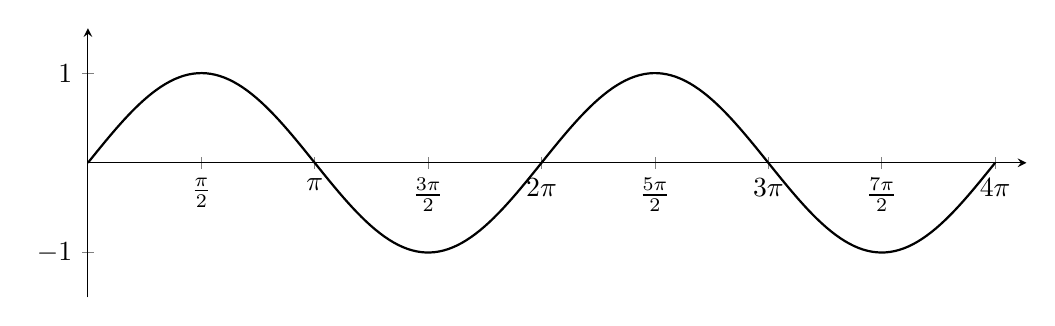
\begin{tikzpicture}
    \begin{axis}[
        Axis Style,
        xtick={
            -6.28318, -4.7123889, -3.14159, -1.5708,
            1.5708, 3.14159, 4.7123889, 6.28318, 7.85398,
            9.42478, 10.99558, 12.56638
        },
        xticklabels={
            $-2\pi$, $-\frac{3\pi}{2}$, $-\pi$, $-\frac{\pi}{2}$,
            $\frac{\pi}{2}$, $\pi$, $\frac{3\pi}{2}$, $2\pi$,
            $\frac{5\pi}{2}$, $3\pi$, $\frac{7\pi}{2}$, $4\pi$
        }]
    \addplot [mark=none, thick] {sin(deg(x))};
    \end{axis}
    \end{tikzpicture}
    \caption{$f(x)=sen(x)$}
    \label{fig:senx}
\end{figure}

\begin{figure}[H]
    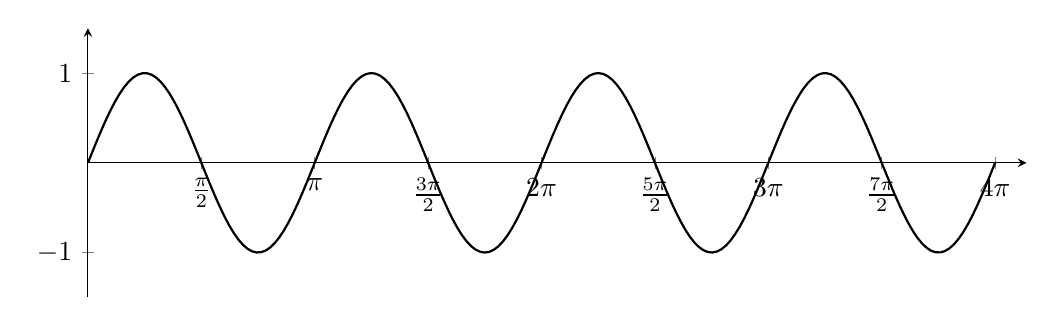
\begin{tikzpicture}
    \begin{axis}[
        Axis Style,
        xtick={
            -6.28318, -4.7123889, -3.14159, -1.5708,
            1.5708, 3.14159, 4.7123889, 6.28318, 7.85398,
            9.42478, 10.99558, 12.56638
        },
        xticklabels={
            $-2\pi$, $-\frac{3\pi}{2}$, $-\pi$, $-\frac{\pi}{2}$,
            $\frac{\pi}{2}$, $\pi$, $\frac{3\pi}{2}$, $2\pi$,
            $\frac{5\pi}{2}$, $3\pi$, $\frac{7\pi}{2}$, $4\pi$
        }]
    \addplot [mark=none, thick] {sin(deg(2*x))};
    \label{sen2x}
    \end{axis}
    \end{tikzpicture}
    \caption{$f(x)=sen(2x)$}
    \label{fig:sen2x}
\end{figure}

Assim, temos duas funções periódicas de período $T = 2\pi$, vale notar que o período mínimo 
de $f(x)$, $T_f = 2\pi$, é maior que o período mínimo de $g(x)$, $T_g = \pi$, mas
que ambas as funções tem o período em comum de $T = 2\pi$. Para somar essas duas
funções, basta somar o valor de $f(x)$ para cada valor de x ao valor de $g(x)$ para 
cada valor de x. Então, teremos o seguinte:
\begin{figure}[H]
    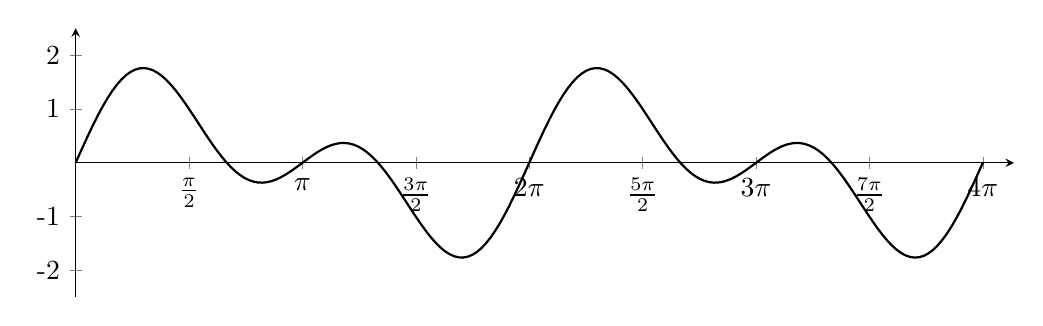
\begin{tikzpicture}
    \begin{axis}[
        Axis Style,
        ymin=-2.5,
        ymax=2.5,
        ytick={-2,-1,0,1,2},
        yticklabels={-2,-1,0,1,2},
        xtick={
            -6.28318, -4.7123889, -3.14159, -1.5708,
            1.5708, 3.14159, 4.7123889, 6.28318, 7.85398,
            9.42478, 10.99558, 12.56638
        },
        xticklabels={
            $-2\pi$, $-\frac{3\pi}{2}$, $-\pi$, $-\frac{\pi}{2}$,
            $\frac{\pi}{2}$, $\pi$, $\frac{3\pi}{2}$, $2\pi$,
            $\frac{5\pi}{2}$, $3\pi$, $\frac{7\pi}{2}$, $4\pi$
        }]
    \addplot [mark=none, thick] {sin(deg(x)) + sin(deg(2*x))};
    \label{sen2x}
    \end{axis}
    \end{tikzpicture}
    \caption{Somando duas funções de mesmo período}
    \label{fig:addExp}
\end{figure}

É possível ver que, a função $f(x)$ possui um período mínimo maior que a função $g(x)$,
assim, \textbf{a função resultante é uma função de período mínimo $T = 2\pi$}, a 
subtração funciona de forma semelhante.\\

Agora podemos afirmar que a soma e a diferença de duas funções 
periódica de período T é também uma função periódica com período T, onde
T é o maior período entre as funções.\\

E quanto à multiplicação e à divisão? Podemos afirmar o mesmo?\\

A resposta é sim, funciona de forma semelhante da soma e da subtração, multiplicando
os valores $f(x)$ por $g(x)$, para todo x. Ficamos com seguinte:
\begin{figure}[H]
    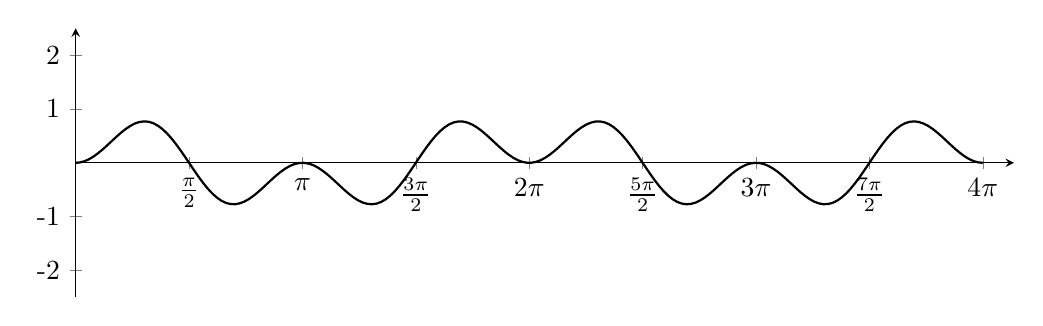
\begin{tikzpicture}
    \begin{axis}[
        Axis Style,
        ymin=-2.5,
        ymax=2.5,
        ytick={-2,-1,0,1,2},
        yticklabels={-2,-1,0,1,2},
        xtick={
            -6.28318, -4.7123889, -3.14159, -1.5708,
            1.5708, 3.14159, 4.7123889, 6.28318, 7.85398,
            9.42478, 10.99558, 12.56638
        },
        xticklabels={
            $-2\pi$, $-\frac{3\pi}{2}$, $-\pi$, $-\frac{\pi}{2}$,
            $\frac{\pi}{2}$, $\pi$, $\frac{3\pi}{2}$, $2\pi$,
            $\frac{5\pi}{2}$, $3\pi$, $\frac{7\pi}{2}$, $4\pi$
        }]
    \addplot [mark=none, thick] {sin(deg(x)) * sin(deg(2*x))};
    \end{axis}
    \end{tikzpicture}
    \caption{Multiplicando funções de mesmo período}
    \label{fig:multExp}
\end{figure}

Por mais esquisito que a função fique, podemos observar que a função resultante
permaneceu com o período $T = 2\pi$. Dessa forma, está claro que operações 
de funções que partilham um mesmo período, terá uma função resultante com o mesmo
período.\\

\begin{definicao}
    Seja $f(x)$ e $g(x)$ duas funções periódicas com período em comum $T$, a soma, subtração,
    multiplicação e divisão das duas funções resulta em uma função periódica de 
    mesmo período mínimo é o maior período entre $f(x)$ e $g(x)$.
\end{definicao}

Mais adiante, temos a seguinte propriedade de qualquer função periódica $f(x)$
com período $T$:\\
\begin{definicao}
Se f(x) é integrável em um intervalo de tamanho T,
então é integrável em qualquer outro intervalo de tamanho T, e o valor da integral
é o mesmo\\
\begin{equation}
\label{int_prop1}
    \int_a^{a+T} \! f(x) \, \mathrm{d}x = \int_b^{b+T} \! f(x) \, \mathrm{d}x.
\end{equation}
para qualquer a, b. \\
\label{def:functPer}
\end{definicao}

Essa propriedade é uma consequência imediata da interpretação da integral como
área. Cada integral é igual a área incluida entre a curva $y=f(x)$, o eixo x e
as ordenadas desenhadas nos limites do intervalo, onde áreas acima do eixo x
são tidas como positivas, e áreas abaixo são tidas como negativas. No caso,
as áreas representadas pelas duas integrais são a mesma por causa da propriedade 
de \ref{def:functPer}. A figura \ref{fig:int_area}, a área em \textcolor{blue}{azul} e a
área em \textcolor{red}{vermelho} representam as áreas das integrais da função
periódica $f(x)=sen(4x)+sen(2x)$ de período $T=\pi$ para intervalos de tamanho $\pi$. 
\\
\begin{figure}[H]
    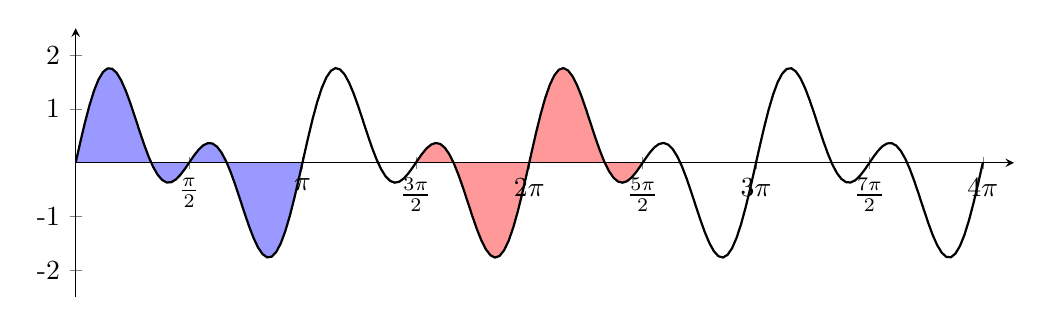
\begin{tikzpicture}
    \begin{axis}[
        Axis Style,
        ymin=-2.5,
        ymax=2.5,
        ytick={-2,-1,0,1,2},
        yticklabels={-2,-1,0,1,2},
        xtick={
            -6.28318, -4.7123889, -3.14159, -1.5708,
            1.5708, 3.14159, 4.7123889, 6.28318, 7.85398,
            9.42478, 10.99558, 12.56638
        },
        xticklabels={
            $-2\pi$, $-\frac{3\pi}{2}$, $-\pi$, $-\frac{\pi}{2}$,
            $\frac{\pi}{2}$, $\pi$, $\frac{3\pi}{2}$, $2\pi$,
            $\frac{5\pi}{2}$, $3\pi$, $\frac{7\pi}{2}$, $4\pi$
        }]
        \addplot[name path=A, mark=none, thick] {sin(deg(4*x)) + sin(deg(2*x))};
        \addplot[name path=B]{0};
        \addplot[blue!40] fill between[of=A and B,
            soft clip={domain=0:3.14159},];
        \addplot[red!40] fill between[of=A and B, 
            soft clip={domain=4.712385:7.853975},];
    \end{axis}
    \end{tikzpicture}
\caption{Observe que ambas as áres são iguais}
\label{fig:int_area}
\end{figure}

Daqui em diante, quando uma função $f(x)$ de período $T$ for integrável, então
ela será integrável em qualquer intervalo de tamanho $T$.

%\chapter{Harmonicos}

A função periódica mais simples é $y = \sin{x}$ e se imaginar constanstes $\mathcal{A} = 1$,
$\omega = 1$ e $\varphi = 0$, podemos reescrever a mesma função da seguinte forma:
\begin{equation}
\label{eq:harm}
    \senoide
\end{equation} 
\\
onde $\mathcal{A}$, $\omega$ e $\varphi$ são constantes. Essa função é chamada de função 
\textit{harmonica} de amplitude $\mathcal{A}$, frequência $\omega$ e fase
inicial $\varphi$. Neste caso, o período dessa harmonica é $T = 2\pi / \omega$
\begin{equation}
\label{harm_ex}
    \mathcal{A}\sin{\left[\omega\left(x+\dfrac{2\pi}{\omega}\right) + \varphi\right]} = \mathcal{A}\sin{[(\omega x + \varphi) + 2\pi]} = \mathcal{A}\sin{(\omega x + \varphi)}
\end{equation}


Agora, vamos definir daqui em diante $\omega > 0$, uma vez que, pela propriedade do seno, 
\mbox{$sen(-a) = - sen (a)$} e examinar o comportamento da função \ref{eq:harm} para 
diferentes valores de amplitude, frequência e fase inicial.
\\
\\


Para $\mathcal{A}=1$, $\omega = 1$ e $\varphi = 0$, temos a curva senóide comum $y = sen x$\\
\\

\begin{figure}[H]
    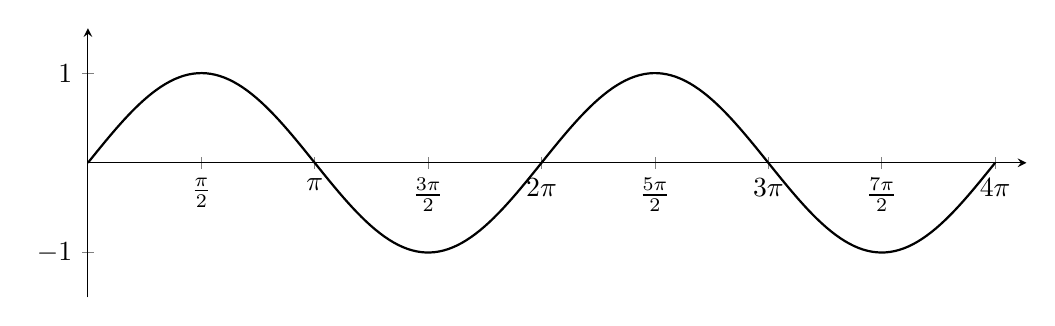
\begin{tikzpicture}
    \begin{axis}[
        Axis Style,
        xtick={
            -6.28318, -4.7123889, -3.14159, -1.5708,
            1.5708, 3.14159, 4.7123889, 6.28318, 7.85398,
            9.42478, 10.99558, 12.56638
        },
        xticklabels={
            $-2\pi$, $-\frac{3\pi}{2}$, $-\pi$, $-\frac{\pi}{2}$,
            $\frac{\pi}{2}$, $\pi$, $\frac{3\pi}{2}$, $2\pi$,
            $\frac{5\pi}{2}$, $3\pi$, $\frac{7\pi}{2}$, $4\pi$
        }]
    \addplot [mark=none, thick] {sin(deg(x))};
    \label{senoide}
    \end{axis}
    \end{tikzpicture}
    \caption{Uma senóide comum}
    \label{fig:senoide}
\end{figure}

Agora considere o seguinte harmonico $y = sen(wx)$ e definir $\omega x = z$, teremos
$y = sen(z)$ cujo gráfico é a curva senóide normal. Portanto, o gráfico de 
$y = sen(\omega x)$ é obtido deformando o gráfico da senóide comum. Por exemplo,
se atribuirmos um $\omega > 1$, teremos uma \textit{compressão} do gráfico da
senóide, então se tivermos $\mathcal{A} = 1$, $\omega = 3$ e $\varphi = 0$, o gráfico 
desse harmonico seria como \ref{fig:compSen} abaixo.

\begin{figure}[H]
    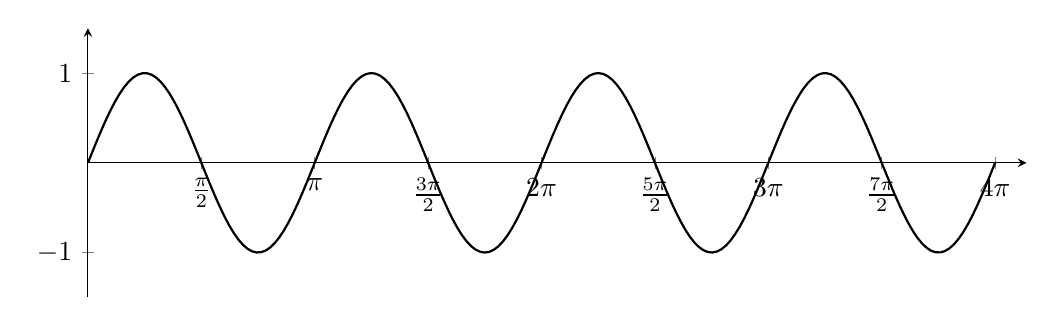
\begin{tikzpicture}
    \begin{axis}[
        Axis Style,
        xtick={
            -6.28318, -4.7123889, -3.14159, -1.5708,
            1.5708, 3.14159, 4.7123889, 6.28318, 7.85398,
            9.42478, 10.99558, 12.56638
        },
        xticklabels={
            $-2\pi$, $-\frac{3\pi}{2}$, $-\pi$, $-\frac{\pi}{2}$,
            $\frac{\pi}{2}$, $\pi$, $\frac{3\pi}{2}$, $2\pi$,
            $\frac{5\pi}{2}$, $3\pi$, $\frac{7\pi}{2}$, $4\pi$
        }]
    \addplot [mark=none, thick] {sin(deg(2*x))};
    \end{axis}
    \end{tikzpicture}
    \caption{Compressão de uma senóide}
    \label{fig:compSen}
\end{figure}

Ou seja, tivemos uma ``compressão" da curva senóide original ao setar $\omega = 2$,
sendo assim sempre que tivermos um $\omega > 1$, teremos uma propocionalmente
\textbf{menor}, neste caso $T = 2\pi / \omega = 2\pi / 3$.

Por outro lado, se atribuirmos um $\omega < 1$, teríamos uma \textit{expansão}
do gráfico da senóide, então se para $\mathcal{A} = 1$, $\omega = 1/4$ e $\varphi = 0$,
o gráfico seria:
\begin{figure}[H]
    \begin{tikzpicture}
    \begin{axis}[
        Axis Style,
        xtick={
            -6.28318, -4.7123889, -3.14159, -1.5708,
            1.5708, 3.14159, 4.7123889, 6.28318, 7.85398,
            9.42478, 10.99558, 12.56638
        },
        xticklabels={
            $-2\pi$, $-\frac{3\pi}{2}$, $-\pi$, $-\frac{\pi}{2}$,
            $\frac{\pi}{2}$, $\pi$, $\frac{3\pi}{2}$, $2\pi$,
            $\frac{5\pi}{2}$, $3\pi$, $\frac{7\pi}{2}$, $4\pi$
        }]
    \addplot [mark=none, thick] {sin(deg((x/2))};
    \end{axis}
    \end{tikzpicture}
    \caption{Expansão de uma senóide}
    \label{fig:expSen}
\end{figure}

Assim, teremos uma "expansão" do gráfico da curva senóide original ao setar $\omega < 1$,
e uma função com período \textbf{maior} com $\omega < 1$, neste caso 
\mbox{$T = 2\pi/\omega = \dfrac{2\pi}{1/2} = 4\pi$}.

Agora considere o harmonico $y = sen(\omega x + \varphi)$ e definir $\omega x + \varphi = \omega z$,
para que $x = z - \varphi/\omega$. Como já sabemos o gráfico de $sen(\omega z)$, o gráfico 
de $y = sen(\omega x + \varphi)$ é obtido deslocando o gráfico de $y = sen(\omega x)$ ao
longo do eixo x por $-\varphi/\omega$. Então, dado $\mathcal{A} = 1$, $\omega = 1$ e $\varphi = 1/2$,
teremos a curva que representa o $cos(x)$

\begin{figure}[H]
    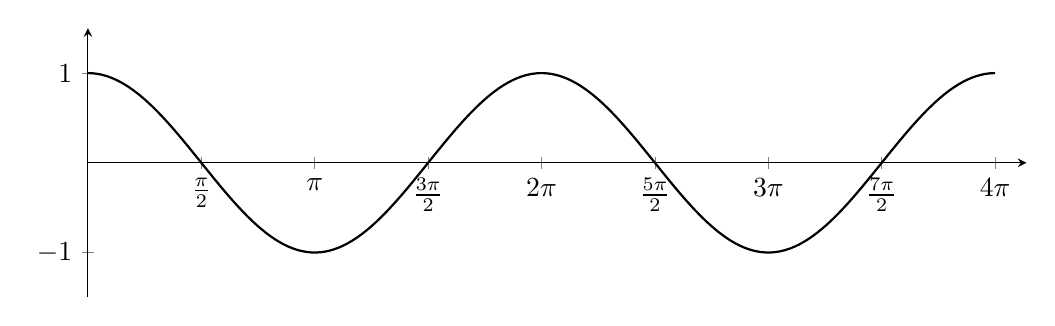
\begin{tikzpicture}
    \begin{axis}[
        Axis Style,
        xtick={
            -6.28318, -4.7123889, -3.14159, -1.5708,
            1.5708, 3.14159, 4.7123889, 6.28318, 7.85398,
            9.42478, 10.99558, 12.56638
        },
        xticklabels={
            $-2\pi$, $-\frac{3\pi}{2}$, $-\pi$, $-\frac{\pi}{2}$,
            $\frac{\pi}{2}$, $\pi$, $\frac{3\pi}{2}$, $2\pi$,
            $\frac{5\pi}{2}$, $3\pi$, $\frac{7\pi}{2}$, $4\pi$
        }]
    \addplot [mark=none, thick] {sin(deg(x+(pi/2)))};
    \end{axis}
    \end{tikzpicture}
    \caption{Deslocamento da senóide}
    \label{fig:deslocSen}
\end{figure}

que nada mais é que a curva senóide deslocada para esquerda.\\
\\
Finalmente, o harmonico \senoide é obtido do harmonico $y = sen(\omega x + \varphi)$
multiplicando todas as ordenadas por $\mathcal{A}$, então dado $\mathcal{A} = 2$, $\omega = 1$ e $\varphi = 0$,
temos

\begin{figure}[H]
    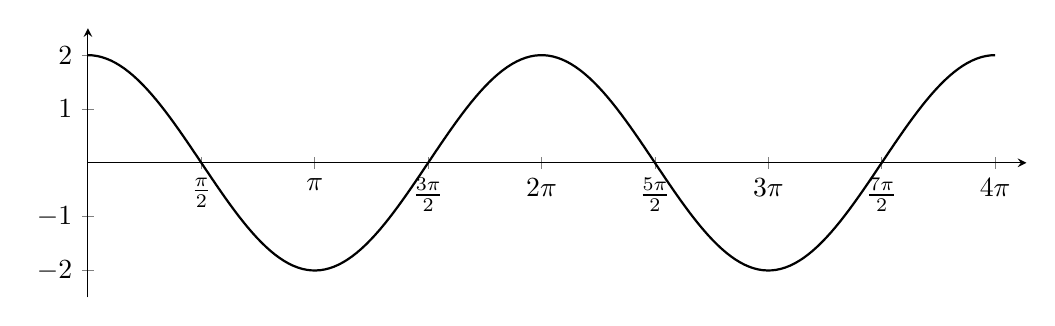
\begin{tikzpicture}
    \begin{axis}[
        Axis Style,
        ymin=-2.5,
        ymax=2.5,
        ytick={-2,-1,0,1,2},
        xtick={
            -6.28318, -4.7123889, -3.14159, -1.5708,
            1.5708, 3.14159, 4.7123889, 6.28318, 7.85398,
            9.42478, 10.99558, 12.56638
        },
        xticklabels={
            $-2\pi$, $-\frac{3\pi}{2}$, $-\pi$, $-\frac{\pi}{2}$,
            $\frac{\pi}{2}$, $\pi$, $\frac{3\pi}{2}$, $2\pi$,
            $\frac{5\pi}{2}$, $3\pi$, $\frac{7\pi}{2}$, $4\pi$
        }]
    \addplot [mark=none, thick] {2*sin(deg(x+(pi/2)))};
    \end{axis}
    \end{tikzpicture}
    \caption{Ampliação da senóide}
    \label{fig:ampSen}
\end{figure}

Portanto, podemos resumir tudo isso no seguinte:\\
\begin{definicao}
    O gráfico de uma harmonica é obtido do gráfico da curva senóide 
    comum por uma compressão (ou expansão) uniforme ao longo dos eixos,
    mais um deslocamento ao longo do eixo x, e é dado pela equação \ref{eq:harm}
\end{definicao}


Assim, podemos utilizar uma conhecida fórmula matemática para derivar
o seguinte:\\
\begin{equation}
    \mathcal{A}sen(\omega x + \varphi) = \mathcal{A}(cos(\omega x)sen(\varphi) + sen(\omega x)cos(\varphi)
\end{equation}
Disso, temos\\
\begin{equation}
    a = \mathcal{A}sen(\varphi)\text{\hspace{10pt},\hspace{10pt}}b = \mathcal{A}cos(\varphi)
\label{eq:ab_harm}
\end{equation}
e então podemos dizer que todo harmonico pode ser representado na forma
\begin{equation}
    y = a \hspace{1pt}cos(\omega x) + b\hspace{1pt}sen(\omega x)
\label{eq:harmSimpl}
\end{equation}
\\
Do mesmo jeito que uma função com a forma \ref{eq:harmSimpl} é um harmonico também. 
Para provar isso, basta resolver \ref{eq:ab_harm} para $a$ e $b$. Temos
\begin{equation}
    \begin{split}
        A = \sqrt{a^2 + b^2}\hspace{5pt},\hspace{10pt} &sen(\varphi) = \dfrac{a}{A} = \dfrac{a}{\sqrt{a^2 + b^2}}\\
        e\hspace{10pt} & cos(\varphi) = \dfrac{b}{A} = \dfrac{b}{\sqrt{a^2 + b^2}}
    \end{split}
\end{equation} 
do qual $\varphi$ pode ser encontrado.\\

Assim, podemos escrever os harmonicos na forma \ref{eq:harmSimpl}. Na Figura \ref{fig:ampSen},
o harmonico pode ser escrito na forma\\
\begin{equation}
    y = \sqrt{2}\cos{3x}+\sin{3x}
\end{equation} 
e a notação dada pela equação \ref{eq:harmSimpl} será usada daqui em diante.\\
\\
Também será conviniente explicitar o período $T$ em \ref{eq:harmSimpl}. Se definirmos
$T = 2l$, então, como $T = 2\pi/\omega$, temos
\begin{equation}
    \notag
    \omega = \dfrac{2\pi}{T}=\dfrac{\pi}{l}
\end{equation}
e assim, o harmonico com período $T=2l$ pode ser escrito da seguinte forma\\
\begin{equation}
    a\cos{\dfrac{\pi x}{l}} + b\sin{\dfrac{\pi x}{l}}
\end{equation}

%\chapter{Polinômios trigonométricos e séries}
Dado o período $T=2l$, considere os harmonicos\\
\begin{equation}
    a_k\cos{\dfrac{\pi kx}{l}} + b_k\sin{\dfrac{\pi kx}{l}},\text{\hspace{5pt}para k = 1,2,3,...}
\end{equation}
\\
Com frequencia $\omega_k = k\pi/l$ e períodos $T_k = \dfrac{2\pi}{\omega_k} = \dfrac{2l}{k}$. 
Uma vez que 
\begin{equation}
\notag
    T = 2l = kT_k
\end{equation}  
\\
\textbf{o número $T=2l$ é simultaneamente o período de todos os harmonicos},
pois um múltiplo de um período é também um período (Sec 1). Então, toda soma na 
forma\\
\begin{equation}
    s_n(n) = \mathcal{A} + \sum\limits_{k=1}^{n}(a_k\cos{\dfrac{k\pi x}{l} + b_k\sin{\dfrac{k\pi x}{l}}})
\end{equation}
\\
é uma função de período $2l$, uma vez que é uma soma de funções de período 
$2l$. Vale notar que $A$ é uma constante e não afeta a periodicidade da função,
inclusive é possível considerar que uma constante é uma função periódica, onde 
qualquer valor pode ser um período.\\
\\
Essa função $s_n(x)$ é chamada  de \textbf{polinômio trigonométrico de ordem n}(
e período $2l$).\\
\\
Por mais que seja a soma de vários harmonicos, um polinômio trigonométrico pode 
ser usado para representar uma função de natureza muito mais complexa que a 
de um harmonico. E geralmente é o caso. Escolhendo as constantes corretamente,
podemos formar funções com gráficos bem diferentes de um simples harmonico.
\\
Na primeira Figura \ref{fig:periodExp}, o polínomio que representa aquele gráfico é\\
\begin{equation}
    y = \sin{x} + \dfrac{1}{2}\sin{2x} + \dfrac{1}{4}\sin{3x}
\end{equation}
\\
Facilmente verificado com algum software de plot de função.\\
\\

A \textbf{série trigonométrica infinita}\\ 
\begin{equation}
    f(x) = A + \sum\limits_{k=1}^{\infty}(a_k\cos{\dfrac{k\pi x}{l}} + b_k\sin{\dfrac{k\pi x}{l}})
\label{eq:serie_inf}
\end{equation}
também representa uma função de período $2l$. As funções como \ref{eq:serie_inf} podem
ser usadas para representar fenômenos de origem muito mais complexa que um polinomio.

Sendo assim, o gráfico de uma função periódica $f(x)$ pode ser obtido através da 
sobreposição de todos os harmonicos que o compõe, i.e., pode ser representado
como uma soma de harmonicos simples.
Então a pergunta que fica é:\\
\textit{Qualquer função que tenha período 2l pode ser representado por uma soma de séries 
trigonométricas?}\\
\\
A resposta é sim, e na realidade, é possível ser usado em grande quantidade de problemas!
Diversos outros fenômenos podem ser ser representado por uma série trigonométrica.
\\
\\  

\textbf{Se}
\begin{equation}
    f(x) = A + \sum\limits_{k=1}^{\infty}(a_k\cos{\dfrac{k\pi x}{l}} + b_k\sin{\dfrac{k\pi x}{l}})
\label{eq:serieLonga}
\end{equation}

\textbf{Então}, podemos definir, por comodidade, que $\dfrac{\pi x}{l} = t$ ou que $x = \dfrac{tl}{\pi}$,
assim teremos\\
\begin{equation}
    g(t) = f(tl/\pi) = A + \sum\limits_{k=1}^{\infty}(a_k\cos{kt} + b_k\sin{kt})
\label{eq:serieSimples}
\end{equation}
\\
onde os harmonicos dessa série tenham período $2\pi$. 

É possível verificar que se a função $f(x)$ de período $2l$ possui a expansão 
\ref{eq:serieLonga}, então a função $g(x)$ de período $2\pi$ possui a expansão 
\ref{eq:serieSimples}, e que o contrário é verdadeiro também. 

Por ser mais legível, daqui em diante usaremos a expansão \ref{eq:serieSimples} 
e ao final faremos a tradução para o mais genérico \ref{eq:serieLonga}.\\

%\section{ Uma terminologia mais precisa}
Agora vamos introduzir a uma terminologia mais precisa e relembrar alguns fatos
de cálculo integral e diferencial. Quando dizemos que $f(x)$ é integrável no 
intervalo [a,b], siginifica que a integral\\
\begin{equation}
\label{int}
    \int_{a}^{b}f(x)dx 
\end{equation}
(que pode ser imprópria) existe no sentido elementar. Portanto, nossas funções 
integráveis $f(x)$ sempre serão contínuas ou com finitas descontinuidades no 
intervalo [a,b], no qual a função pode ser limitada ou não.\\
\\
Em cursos de cálculo integral, primeiro se prova que a função possui um número
finito de descontinuidades dentro de um intervalo, então se a integral\\
\\
\begin{equation}
    \int_{a}^{b}|f(x)|dx 
\end{equation} 
\\
existe, então \ref{int} também existe. Neste caso, a função $f(x)$ é tida como
uma função \textbf{absolutamente integrável}. (Vale notar que o inverso pode não
ser verdadeiro).\\
\\
\textbf{Propriedade 1}\\
Se $f(x)$ é uma função absolutamente integrável e $g(x)$ é uma função integrável
limitada, então o produto $f(x)g(x)$ é uma função absolutamente integrável também.
\\
\\
A seguinte regra de integração por partes é válida:\\
\\
\textit{Seja f(x) e g(x) contínuas em [a,b], mas talvez não diferençiavel
em um número finito de pontos. Portanto se f'(x) e g'(x) são absolutamente 
integráveis, então temos:}\\
\begin{equation}
    \int_{a}^{b}f(x)g'(x) dx = [f(x)g(x)]_{a}^{b} - \int_{a}^{b}f'(x)g(x) dx
\end{equation}

Outro resultado familiar é o fato que se as funções $f_1(x), f_2(x), ..., f_n(x)$
são integráveis no intervalo [a,b], então a soma deles também é integrável.\\
\begin{equation}
\label{43}
    \int_{a}^{b}[\sum\limits_{k=1}^{n}f(x)]dx = \sum\limits_{k=1}^{n}\int_{a}^{b}f(x)dx
\end{equation}

Agora considere uma série infinita de funções:\\
\begin{equation}
\label{44}
    f_1(x), f_2(x), f_3(x), ... = \sum\limits_{k=1}^{\infty}f_k(x)
\end{equation}
\\
Uma série desse tipo é dita convergente se para um dado valor de x,
suas somas parciais:\\
\begin{equation}
    s_n(x) = \sum\limits_{k=1}^{n}f_k(x)\text{, para n = 1, 2, 3, ...}
\end{equation}
\\
tiverem um limite finito:\\
\begin{equation}
    s(x) = \lim_{x\to\infty} s_n(x)
\end{equation}
\\
$s(x)$ é dita ser a soma da série e, obviamente, é uma função de $x$.\\
\\
Se a série converge para todo x no intervalo [a,b], então sua soma $s(x)$
é definida em todo o intervalo [a,b].\\
\\
Agora perguntamos se a formula \ref{43} pode ser extendida para o caso de 
uma série convergente de funções integráveis no intervalo [a,b], i.e.,
a fórmula abaixo é válida?\\
\begin{equation}
\label{45}
    \int_{a}^{b}[\sum\limits_{k=1}^{\infty}f(x)]dx = \int_{a}^{b}s(x) dx = \sum\limits_{k=1}^{\infty}\int_{a}^{b}f_k(x) dx
\end{equation}
\\
Em outras palavras, a série pode ser integrada termo a termo?\\
\\
\ref{45} nem sempre é válida, simplesmente pela série de funções integráveis,
ou até mesmo contínua pode, se quer, ter uma soma integrável. Um problema parecido 
surge com relação a possibilidade de diferenciação termo a termo da série.
E agora vamos descartar uma importante classe de séries de função para o qual 
essas operações podem ser aplicadas.\\
\\
A série \ref{44} é dita ser uniformemente convergente em um intervalo [a,b] se
para um número positivo qualquer $\varepsilon$, existe um número $N$ tal que a
desigualdade abaixo seja verdadeira para todo $n \geq N$ e para todo x no 
intervalo [a,b].\\
\begin{equation}
    |s(x) - s_n(x)| \leq \varepsilon
\end{equation}
\\
Portanto, convergência uniforme significa que para um $n$ suficientemente 
grande e para todo $x$ no intervalo, o gráfico da soma de séries $s(x)$ e o 
gráfico da soma parcial $s_n(x)$, estão $\varepsilon$ distantes uma da outra,
desse jeito, ambas as curvas estarão \textit{uniformemente perto} uma da outra.\\
\\
\textit{Importante Notar:}
Não é qualquer série que converge no intervalo [a,b] e, também, convere uniformemente
no mesmo intervalo.\\
\\
\textbf{gap} 
\\
O teste a seguir é um teste muito útil e simples para a convergencia uniforme
de uma série de funções (Weierstrass M-Test):\\
\textit{
    Se a série infinita de números \\
    \begin{equation}
        M_1 + M_2 + M_3 + ... + M_k + ...
    \end{equation}
    \\
    \\
    convergir e, se para algum x no intervalo [a,b], nós tivermos $|f_k(x)| \leq M_k$
    de um certo k em diante, então a série \ref{43} converge uniformemente ( e 
    absolutamente) no intervalo [a,b].
} 
\\
\textbf{gap}\\
\\
Os seguintes teoremas são válidos:

\newtheorem{teo1}{Teorema}
\begin{teo1}
    Se os termos da série \ref{44} são contínuos em [a,b] e se a
    série converge uniformemente em [a,b], então:\\
    a) A soma da série é contínua\\
    b) A soma pode ser integrada termo a termo
\end{teo1}

\newtheorem{teo2}{Teorema}
\begin{teo2}
    Se a série \ref{44} converge, e se os termos da série são diferenciáveis
    e se a série:\\
    \begin{equation}
        f_1^{'}(x) + f_2^{'}(x) + f_3^{'}(x) + ... = \sum\limits_{k=1}^{\infty}f_k^{'}(x)
    \end{equation}
    é uniformemente convergente em [a,b], então\\
    \begin{equation}
        (\sum\limits_{k=1}^{\infty} f(x))^{'} = s^{'}(x) = \sum\limits_{k=1}^{\infty}f_k^{'}(x)
    \end{equation}
    i.e., a série \ref{44} pode ser diferenciada termo a termo.
\end{teo2}

\chapter{Revisão de trigonometria}

Um \textit{sistema básico trigonométrico} significa um sistema de funções como 
as de \ref{eq:51} que possuem um período $T=2\pi$\\
\begin{equation}
    1, cos(x), sen(x), cos(2x), sen(2x), ... 
\label{eq:51}
\end{equation}
\\
Com base nessas funções, vamos mostrar algumas funções que irão auxiliar mais
adiante.\\


Para um inteiro $n \neq 0$, temos\\
\begin{definicao}
    \label{def:52}
    A integral definida em um intervalo de tamanho $T=2\pi$ da função $f(x)=sen(x)$ é sempre 
    igual a zero. O mesmo vale para $g(x)=cos(x)$.
    \begin{equation}
        \begin{split}
            \int_{0}^{2\pi}cos(nx)dx & = \left[\dfrac{sen(nx)}{n}\right]_{0}^{2\pi} = 0\\
            \int_{0}^{2\pi}sen(nx)dx & = \left[\dfrac{-cos(nx)}{n}\right]_{0}^{2\pi} = 0
        \end{split}
    \end{equation}
\end{definicao}

Se desenharmos o gráfico das funções $sen(x)$ e $cos(x)$, fica evidente que sua 
integral é zero. Na figura \ref{fig:intSen}, a parte em \textcolor{red}{vermelho} 
é positiva e a parte em \textcolor{blue}{azul} é negativa, e como ambas são iguais,
a área total das funções $sen(x)$ e $cos(x)$ no intervalo $[0:2\pi]$ é zero.
\begin{figure}[H]
    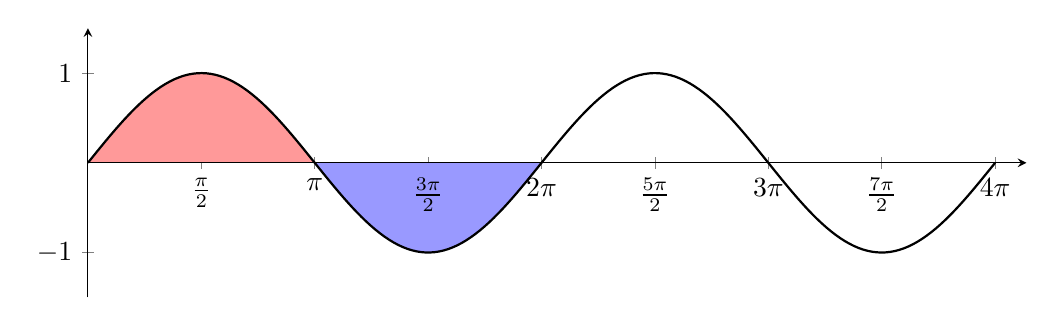
\begin{tikzpicture}
    \begin{axis}[
        Axis Style,
        xtick={
            -6.28318, -4.7123889, -3.14159, -1.5708,
            1.5708, 3.14159, 4.7123889, 6.28318, 7.85398,
            9.42478, 10.99558, 12.56638
        },
        xticklabels={
            $-2\pi$, $-\frac{3\pi}{2}$, $-\pi$, $-\frac{\pi}{2}$,
            $\frac{\pi}{2}$, $\pi$, $\frac{3\pi}{2}$, $2\pi$,
            $\frac{5\pi}{2}$, $3\pi$, $\frac{7\pi}{2}$, $4\pi$
        }]
        \addplot[name path=A, mark=none, thick] {sin(deg(x))};
        \addplot[name path=B]{0};
        \addplot[red!40] fill between[of=A and B,
            soft clip={domain=0:3.14159},];
        \addplot[blue!40] fill between[of=A and B, 
            soft clip={domain=3.14159:3.14159+3.14159},];
    \end{axis}
    \end{tikzpicture}
    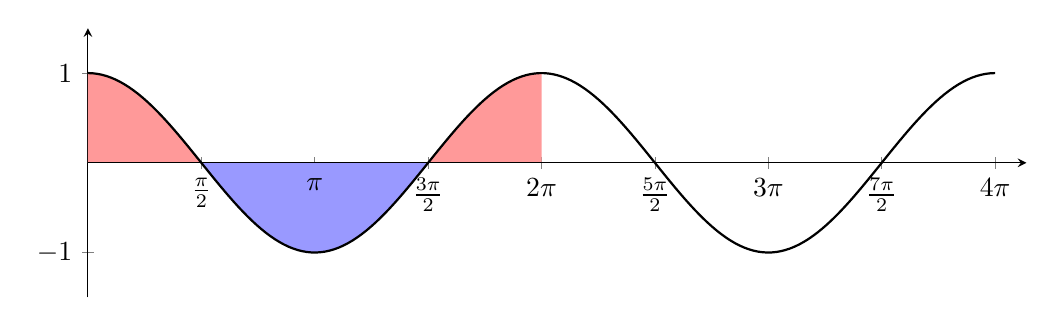
\begin{tikzpicture}
    \begin{axis}[
        Axis Style,
        xtick={
            -6.28318, -4.7123889, -3.14159, -1.5708,
            1.5708, 3.14159, 4.7123889, 6.28318, 7.85398,
            9.42478, 10.99558, 12.56638
        },
        xticklabels={
            $-2\pi$, $-\frac{3\pi}{2}$, $-\pi$, $-\frac{\pi}{2}$,
            $\frac{\pi}{2}$, $\pi$, $\frac{3\pi}{2}$, $2\pi$,
            $\frac{5\pi}{2}$, $3\pi$, $\frac{7\pi}{2}$, $4\pi$
        }]
        \addplot[name path=C, mark=none, thick] {sin(deg(x +1.5708))};
        \addplot[name path=D]{0};
        \addplot[red!40] fill between[of=C and D,
            soft clip={domain=0:1.5708},];
        \addplot[blue!40] fill between[of=C and D, 
            soft clip={domain=1.5708:1.5708+3.14159},];
        \addplot[red!40] fill between[of=C and D,
            soft clip={domain=1.5708+3.14159:6.28318},];            
    \end{axis}
    \end{tikzpicture}    
\caption{A integral como área das funções $f(x)=sen(x)$ e $g(x)=cos(x)$}
\label{fig:intSen}
\end{figure}

Também podemos afirmar que\\
\begin{definicao}
    \label{def:53}
    A integral definida em um intervalo de tamanho $T=2\pi$ da função $f(x)=sen^2(x)$
    é sempre a metade do período. O mesmo vale para $g(x)=cos(x)$.
    \begin{equation}
        \begin{split}
            \int_{0}^{2\pi}cos^2(nx)dx & = \int_{0}^{2\pi}\dfrac{1 + cos(2nx)}{2} dx = \pi\\
            \int_{0}^{2\pi}sen^2(nx) dx & = \int_{0}^{2\pi}\dfrac{1 - cos(2nx)}{2} dx = \pi
        \end{split}
    \end{equation}
\end{definicao}

Olhando para o gráfico das funções $f(x)=sen^2(x)$ e $g(x)=cos^2(x)$, representado na figura
\ref{fig:intSenQuad} abaixo, fica claro que a parte que antes era negativa, torna-se positiva
e a parte positiva permanece igual.

\begin{figure}[H]
    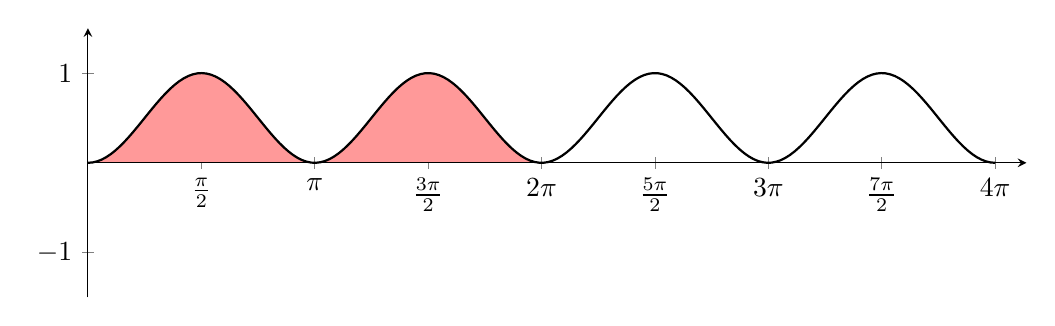
\begin{tikzpicture}
    \begin{axis}[
        Axis Style,
        xtick={
            -6.28318, -4.7123889, -3.14159, -1.5708,
            1.5708, 3.14159, 4.7123889, 6.28318, 7.85398,
            9.42478, 10.99558, 12.56638
        },
        xticklabels={
            $-2\pi$, $-\frac{3\pi}{2}$, $-\pi$, $-\frac{\pi}{2}$,
            $\frac{\pi}{2}$, $\pi$, $\frac{3\pi}{2}$, $2\pi$,
            $\frac{5\pi}{2}$, $3\pi$, $\frac{7\pi}{2}$, $4\pi$
        }]
        \addplot[name path=A, mark=none, thick] {sin(deg(x))*sin(deg(x))};
        \addplot[name path=B]{0};
        \addplot[red!40] fill between[of=A and B,
            soft clip={domain=0:6.28318},];
    \end{axis}
    \end{tikzpicture}
    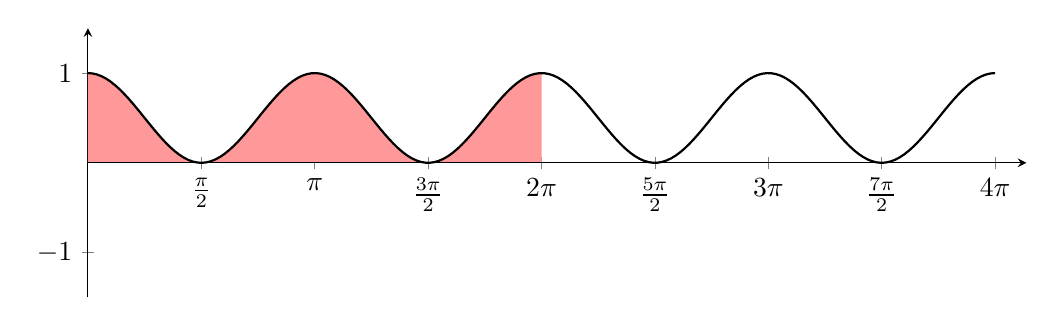
\begin{tikzpicture}
    \begin{axis}[
        Axis Style,
        xtick={
            -6.28318, -4.7123889, -3.14159, -1.5708,
            1.5708, 3.14159, 4.7123889, 6.28318, 7.85398,
            9.42478, 10.99558, 12.56638
        },
        xticklabels={
            $-2\pi$, $-\frac{3\pi}{2}$, $-\pi$, $-\frac{\pi}{2}$,
            $\frac{\pi}{2}$, $\pi$, $\frac{3\pi}{2}$, $2\pi$,
            $\frac{5\pi}{2}$, $3\pi$, $\frac{7\pi}{2}$, $4\pi$
        }]
        \addplot[name path=C, mark=none, thick] {sin(deg(x +1.5708))*sin(deg(x +1.5708))};
        \addplot[name path=D]{0};
        \addplot[red!40] fill between[of=C and D,
            soft clip={domain=0:6.28318},];           
    \end{axis}
    \end{tikzpicture}    
\caption{A integral como área das funções $f(x)=sen^2(x)$ e $g(x)=cos^2(x)$}
\label{fig:intSenQuad}
\end{figure}

 
Mais adiante, usando fórmulas trigonométricas conhecidas, temos\\
\\
\begin{equation}
\label{eq:54}
    \begin{split}
        cos(\alpha)cos(\beta) & = \dfrac{1}{2}[cos(\alpha + \beta) + cos(\alpha - \beta)]\\
        sen(\alpha)sen(\beta) & = \dfrac{1}{2}[cos(\alpha - \beta) - cos(\alpha + \beta)]
    \end{split}
\end{equation}
\\
para qualquer $n$, $m$.\\
\\
Finalmente, usando a fórmula \\
\begin{equation}
        sen(\alpha)cos(\beta) = \dfrac{1}{2}[\sin{(\alpha + \beta)} + \sin{(\alpha - \beta)}]    
\end{equation}
\\
tiramos o seguinte:\\
\\
\begin{definicao}
    A integral definida em um intervalo de tamanho $T=2\pi$ da função $f(x)=sen(nx)*cos(mx)$
    é sempre igual a zero, para qualquer n, m.
    \begin{equation}
        \int_{0}^{2\pi}\sin{nx}\cos{mx}dx = 0
    \end{equation}
    \label{def:55}
\end{definicao}

A assim como em \ref{def:53}, fica evidente que a área do total da função 
$f(x)=sen(x)*cos(x)$ é igual a zero.
\begin{figure}[H]
    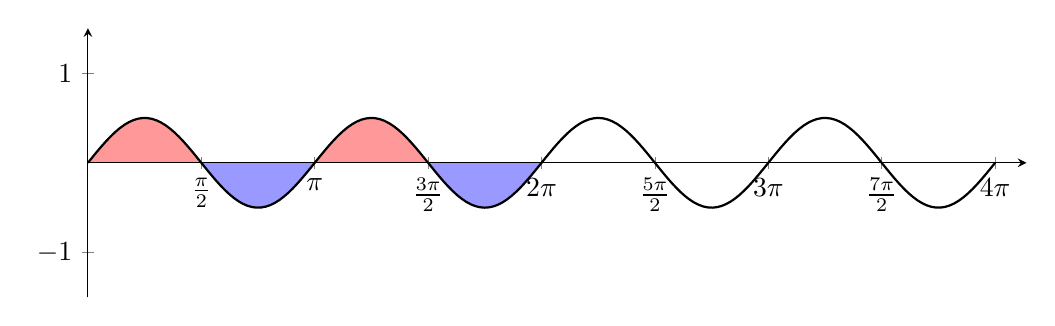
\begin{tikzpicture}
    \begin{axis}[
        Axis Style,
        xtick={
            -6.28318, -4.7123889, -3.14159, -1.5708,
            1.5708, 3.14159, 4.7123889, 6.28318, 7.85398,
            9.42478, 10.99558, 12.56638
        },
        xticklabels={
            $-2\pi$, $-\frac{3\pi}{2}$, $-\pi$, $-\frac{\pi}{2}$,
            $\frac{\pi}{2}$, $\pi$, $\frac{3\pi}{2}$, $2\pi$,
            $\frac{5\pi}{2}$, $3\pi$, $\frac{7\pi}{2}$, $4\pi$
        }]
        \addplot[name path=A, mark=none, thick] {sin(deg(x))*sin(deg(x+1.5708))};
        \addplot[name path=B]{0};
        \addplot[red!40] fill between[of=A and B,
            soft clip={domain=0:1.5708},];
        \addplot[blue!40] fill between[of=A and B,
            soft clip={domain=1.5708:3.14159},];
        \addplot[red!40] fill between[of=A and B,
            soft clip={domain=3.14159:4.7123889},];
        \addplot[blue!40] fill between[of=A and B,
            soft clip={domain=4.7123889:6.28318},];            
    \end{axis}
    \end{tikzpicture}
\caption{A integral como área da função $f(x)=sen(x)*cos(x)$}
\label{fig:intSenCos}
\end{figure}

As fórmulas de \ref{def:52} e \ref{eq:54}, mostram que a integral sobre um intervalo $[0, 2\pi]$
do produto de qualquer duas funções diferentes do sistema \ref{eq:51} desaparece.

Finalmente, definimos
\begin{definicao}
\label{def:56}
    Duas funções $f(x)$ e $g(x)$ são ortogonais em um intervalo $[a,b]$ se
    \begin{equation}
        \int_{a}^{b} f(x)g(x)\hspace{4pt}dx = 0
    \end{equation}
\end{definicao}

Com a definição \ref{def:56}, podemos dizer que os pares de funções em \ref{eq:51} são
ortogonais no intervalo $[0, 2\pi]$.

Como já foi dito na Sec. 1, a integral de uma função periódica é a mesma em
qualquer outro intervalo de mesmo tamanho que o período, no caso $2\pi$.



%\section{Séries de Fourier para funções de período $2\pi$}
Suponha que a função $f(x)$ de período $2\pi$ tenha a seguinte expansão:\\
\begin{equation}
    \label{61}
    f(x) = \dfrac{a_0}{2} + \sum\limits_{k=1}^{\infty}(a_k\cos{kx} + b_k\sin{kx})
\end{equation}
\\
onde, para simplificar para próximas fórmulas, vamos denotar a constante da 
expansão como sendo $\dfrac{a_0}{2}$.\\
\\
Agora, vamos resolver o problema para achar os valores de $a_0, a_k, b_k$, para
k = 1, 2, 3, ..., por um conhecimento em $f(x)$.\\
\\
Para isso, vamos fazer a seguinte suposição:\\
\\
$\to$ A série \ref{61} e a série a seguir podem ser integradas termo a termo, ou seja
a integral das somas é igual a soma das integrais.
\\
\\
Então, integrando \ref{61} no intervalo $[-\pi, \pi]$, ficamos com:\\
\begin{equation}
    \int_{-\pi}^{\pi} f(x)\hspace{5pt}dx = \dfrac{a_0}{2}\int_{-\pi}^{\pi}dx + \sum\limits_{k=1}^{\infty}(a_k\int_{-\pi}^{\pi}\cos{kx}dx + b_k\int_{-\pi}^{\pi}\sin{kx}dx)
\end{equation}
\\
Pela \ref{52}, todas as integrais somem\\
\\
\begin{equation}
    \label{62}
    \int_{-\pi}^{\pi}f(x) dx = \pi a_0
\end{equation}
\\
Agora, vamos multiplicaros dois lados por $\cos{nx}$ e integrar o resultado no 
intervalo $[-\pi, \pi]$, como antes, desta vez temos:\\
\\
\begin{equation}
    \int_{-\pi}^{\pi} f(x)\cos{nx}\hspace{5pt}dx = \dfrac{a_0}{2}\int_{-\pi}^{\pi}\cos{nx}dx + \sum\limits_{k=1}^{\infty}(a_k\int_{-\pi}^{\pi}\cos{kx}\cos{nx}dx + b_k\int_{-\pi}^{\pi}\sin{kx}\cos{nx}dx)
\end{equation}
\\
Pela \ref{52}, todas as integrais desaparecem, com exceção de uma, a de coeficiente $a_n$.\\
\\
\begin{equation}
    \int_{-\pi}^{\pi}\cos^2{nx}dx = \pi
\end{equation}
\\ 
E disso, temos\\
\\
\begin{equation}
\label{63}
    \int_{-\pi}^{\pi}f(x)\cos{nx}dx = a_n\pi
\end{equation}
\\
De mesmo modo\\
\\
\begin{equation}
\label{64}
    \int_{-\pi}^{\pi}f(x)\sin{nx}dx = b_n\pi
\end{equation}
\\
Então, dado \ref{63} e \ref{64}, temos\\
\begin{equation}
\label{eq:65}
    \begin{split}
        a_n &= \dfrac{1}{\pi}\int_{-\pi}^{\pi}f(x)\cos{nx}dx\\
        b_n &= \dfrac{1}{\pi}\int_{-\pi}^{\pi}f(x)\sin{nx}dx
    \end{split}
\end{equation}
\\
Finalmente, se $f(x)$ é integrável e pode ser expandido em uma série trigonométrica,
e se essa série e a série obtida multiplicando por $\cos{nx}$ e $\sin{nx}$ ($n = 1, 2, 3, ...$)
pode ser integrada termo a termo, então os coeficientes $a_n$ e $b_n$ são dados pela
fórmula \ref{eq:65}. Estes coeficientes são conhecidos como \textit{coeficientes de Fourier}
da função $f(x)$, que representa a série trigonométrica conhecida como \textit{Série de
Fourier}.\\
\end{document}

